\pdfinfo{
/ModDate (\pdfcreationdate)                                   
/Producer (pdfLaTeX)}


\documentclass[fleqn,oneside,openany,a4paper,11pt]{book}

\usepackage{color}
\usepackage[utf8]{inputenc}
\usepackage[breaklinks]{hyperref} %
\usepackage{pracadok}
\usepackage{longtable}
\usepackage{array}
\usepackage{geometry}
\usepackage{fancyhdr}
\usepackage{float}

\pdfcompresslevel=9

\def\uwaga#1{}

\begin{document}
\let\s\lstinline
\lstset{inputencoding=utf8, extendedchars=true,literate={ą}{{\k{a}}}1 {ć}{{\'c}}1 {ę}{{\k{e}}}1 {ł}{{\l{}}}1 {ń}{{\'n}}1 {ó}{{\'o}}1 {ś}{{\'s}}1 {ż}{{\.z}}1 {ź}{{\'z}}1 {Ą}{{\k{A}}}1 {Ć}{{\'C}}1 {Ę}{{\k{E}}}1 {Ł}{{\L{}}}1 {Ń}{{\'N}}1 {Ó}{{\'O}}1 {Ś}{{\'S}}1 {Ż}{{\.Z}}1 {Ź}{{\'Z}}1}

% Tytuł
\def\autor{Informatyka Stosowana III rok}
\def\tytul{\textbf{\LARGE Zespołowe Przedsięwzięcie Inżynierskie}}
\def\promotor{~}
\def\miejscerokwydania{Nowy Sącz \today}
\def\nazwauczelni{PAŃSTWOWA WYŻSZA SZKOŁA ZAWODOWA}
\def\imienia{INSTYTUT  TECHNICZNY}
\def\wydzial{Kierunek Informatyka Stosowana}

\thispagestyle{empty}
{
\hbox{}\vskip 0.3\textheight
\hspace{1cm}
\centering
\vbox{
\noindent\textbf{\Huge Regulamin \\ \vspace{0.3cm}turnieju szachowego}\vspace{0.5cm}\\
}
\definecolor{tlo}{rgb}{.7,.7,.7} 
\lstset{language=bash,commentstyle=\scriptsize,backgroundcolor=\color{tlo},%
basicstyle=\scriptsize}

%spis tresci
{\footnotesize\tableofcontents}

\setcounter{chapter}{0}

\textbf{}
\vbox{
\centering	\noindent\textbf{\Huge Regulamin turnieju szachowego}\vspace{0.5cm}}\\
\begin{enumerate}
\item Obowiązują przepisy gry międzynarodowej federacji szachowej (FIDE).
\item Każdy z zawodników powinien się kierować zasadami fair play.
\item Zasady rozgrywki:
\begin{enumerate}
\item Turniej rozgrywany jest w dwóch fazach: grupowej i finałowej.
\item Ilość grup jest zależna od liczby uczestników i ustala ją prowadzący.
\item W fazie grupowej prowadzone są rozgrywki, wedug zasady "każdy z każdym" w danej grupie
\item W fazie finałowej zawodnicy wyłonieni z grup (liczbę osób wychodzących z grup ustala prowadzący) grają między sobą.
\item Jeżeli zawodnicy grali ze sobą w rundzie eliminacyjnej to w finale przyjmuje się wynik rozgrywki z eliminacji
\item Czas trwania turnieju jest ograniczony, podany przez organizatora
\begin{itemize}
\item \textbf{10 minut} na przyjmowanie zgłoszeń(rejestrację), \textbf{10 minut} na losowanie spotkań, \textbf{10 minut} na rozegranie partii, każdy zawodnik ma 5 minut na wykonanie swoich posunięć.
\end{itemize}
\item Zawodnicy mają do dyspozycji zegar analogowy lub cyfrowy z 2 tarczami lub wyświetlaczami umożliwiający odmierzanie czasu rozgrywki dla każdego z zawodników osobno
\item Za zajecie ustalonych przez prowadzącego miejsc w turnieju zawodnicy otrzymują nagrody przewidziane przez organizatora.
\item Jeśli prowadzący ustali, uczestnicy będą mieli obowiązek zapisywać swoje ruchy na przeznaczonych do tego kartach.
\item Każdy stanowisko do gry ma swój numer identyfikacyjny, który obowiązuje przy rozgrywkach.
\item W sali, w której obywa się turniej szachowy zawodnicy jak i widzowie muszą zachować bezwzględną ciszę, aby nie przeszkadzać graczom w rozgrywce.
\item W turnieju obowiązuje punktacja
\begin{itemize}
	\item Zwycięstwo - \textbf{1pkt}, Remis - \textbf{0,5pkt}, Porażka - \textbf{0pkt}
	\item Punkty pomocnicze, wykorzystywane gdy kilku zawodników ma taką samą liczbę punktów głównych, przyznawane po zakończeniu etapu (eliminacji lub finału) według wzoru: suma puktów zawodników z którymi gracz wygrał + połowa sumy punktów z którymi zremisował
\end{itemize}
\end{enumerate}
\item W razie rezygnacji lub dyskwalifikacji zawodnika z turnieju, rozgrywki, które rozegrał nie zostają anulowane, a osoby, które się z nim spotykają w kolejnych rozgrywkach wygrywają walkowerem (otrzymują 1pkt za zwycięstwo)
\item W Sali zostało wydzielone pięć części:
\begin{enumerate}
\item Pierwsza, w której znajdują się tylko i wyłącznie osoby rozgrywające mecz
\item Druga, w której znajdują się widzowie bądź gracze, którzy obecnie nie rozgrywają żadnego spotkania
\item Trzecia, w której znajdują się stanowiska do gry w szachy poza turniejem
\item Czwarta, w której znajdują się gracze oczekujący na mecz
\item Piąta, w której znajduje się tylko i wyłącznie prowadzący turniej szachowy bądź osoby, które za zezwoleniem mogą znajdować się w tej strefie
\end{enumerate}
\item Zawodnicy, którzy nie grają lub czekają na swoją kolej w obrębie sali lub w niedalekiej odległości od niej w wypadku wezwania do rozgrywki powinni w trybie natychmiastowym zgłosić się do udziału w spotkaniu. W wypadku niestawienia się do rozegrania meczu zawodnik zostaję zdyskwalifikowany.
\item W przypadku, gdy:
\begin{itemize}
\item Zawodnik który korzysta z niedozwolonej pomocy lub utrudnia przeprowadzanie rozgrywek  może zostać zdyskwalifikowany z turnieju lub wyproszony z sali przez Prowadzącego.
\item Widz utrudnia przeprowadzanie rozgrywek może zostać wyproszony z sali przez Prowadzącego.
\end{itemize}
\item Udział w turnieju szachowym jest równoznaczny z zaakceptowaniem regulaminu
\end{enumerate}
% początkowy opis projektu
\chapter{Obsługa programu}
Uruchamiamy program
\begin{figure}[H]
	\centering
	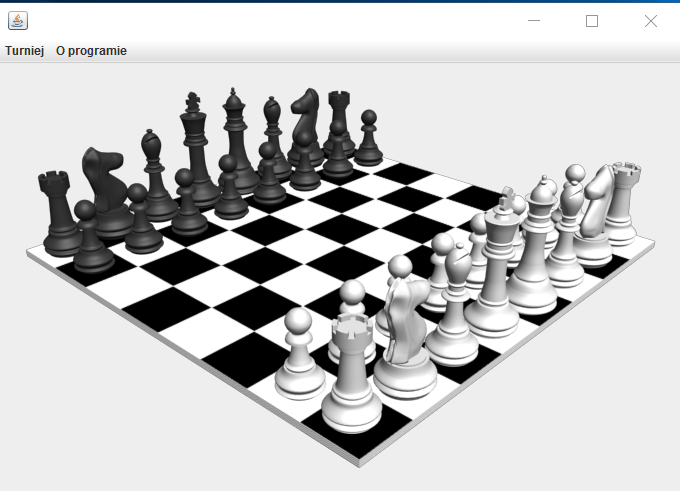
\includegraphics[width=10cm]{fig/1}
	\caption{Główne okno programu}
	\label {fig:glowne_okno_programu} 
\end{figure}
Z menu "Turniej" możemy wybrać opcję lub użyć skrótu klawiaturowego
\begin{figure}[H]
	\centering
	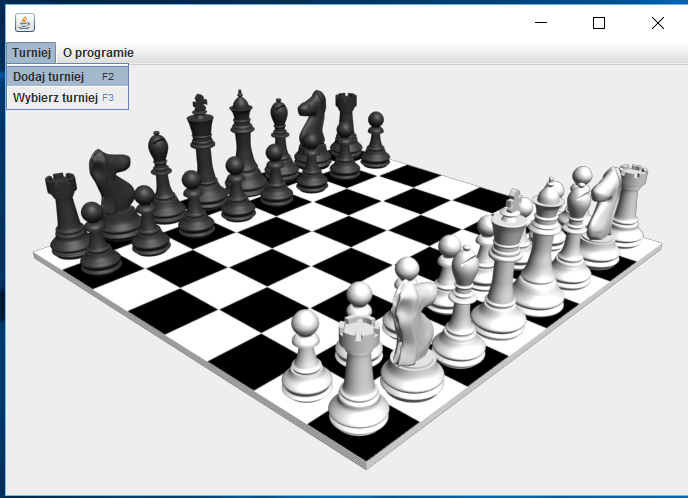
\includegraphics[width=10cm]{fig/2}
	\caption{Wybór turnieju}
	\label {fig:wybor_turnieju} 
\end{figure}
Jeżeli wybierzemy opcję "Dodaj turniej" musimy nadać mu nazwę
\begin{figure}[H]
	\centering
	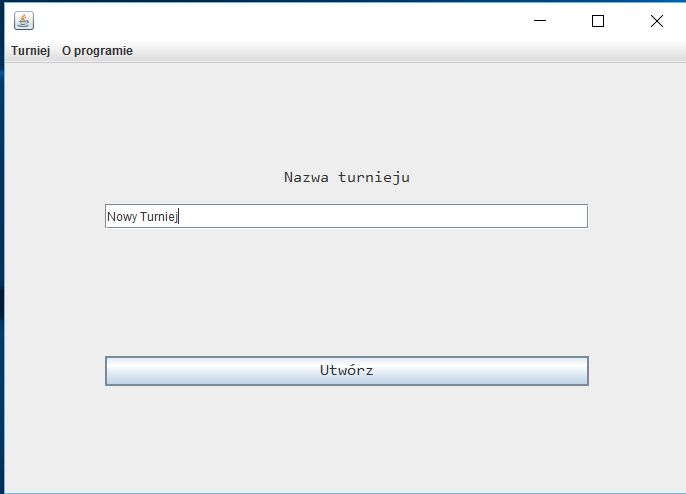
\includegraphics[width=10cm]{fig/3}
	\caption{Wybór nazwy turnieju}
	\label {fig:wybor_nazwy_turnieju} 
\end{figure}
Uczestnika turnieju możemy dodać na 2 sposoby:
\begin{enumerate}
	\item losowo
	\item uzupełniając jego dane
\end{enumerate}
\begin{figure}[H]
	\centering
	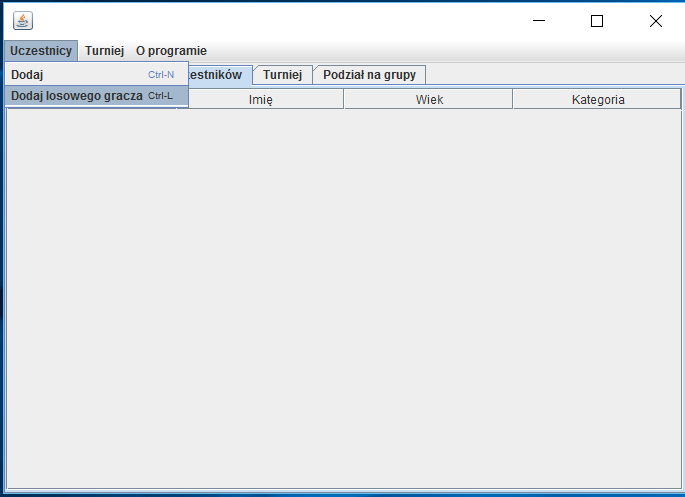
\includegraphics[width=10cm]{fig/4}
	\caption{Dodawanie uczestnika do turnieju}
	\label {fig:dodawanie_uczestnika_do_turnieju} 
\end{figure}
Wpisujemy dane użytkownika, kategorie możemy wybrać z listy
\begin{figure}[H]
	\centering
	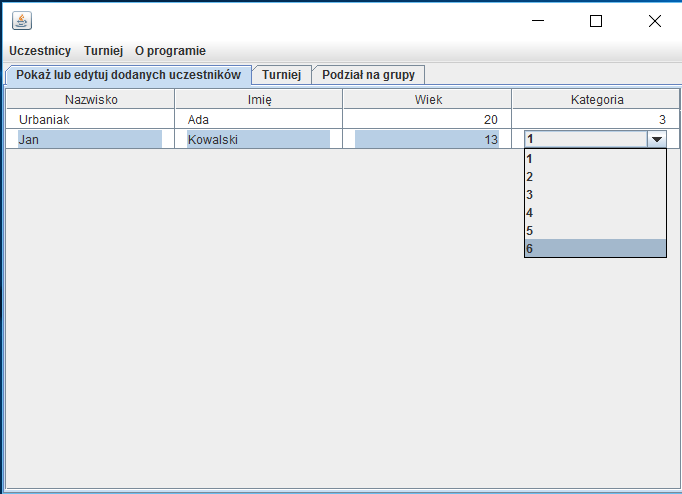
\includegraphics[width=10cm]{fig/5}
	\caption{Wybór kategorii}
	\label {fig:wybor_kategorii} 
\end{figure}
Istnieje możliwość usunięcia zawodnika z listy.\\
Klikamy PPM na wierszu w którym znajdują się dane zawodnika którego chcemy usunąć i wybieramy opcję "usuń" 
\begin{figure}[H]
	\centering
	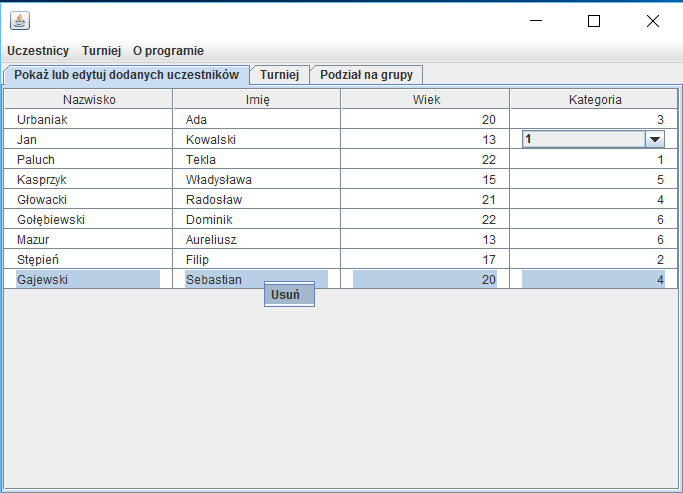
\includegraphics[width=10cm]{fig/6}
	\caption{Usuwanie zawodnika z listy}
	\label {fig:Usuwanie_zawodnika_z_listy} 
\end{figure}
W zakładce turniej możemy ustawic parametry turnieju takie jak:
\begin{enumerate}
	\item nazwa turnieju
	\item rok
	\item czas trwania pojedyńczej rozgrywki - minimum 1 minuta, maksimum 20 minut
	\item ilość drużyn - program wskaże optymalną ilość grup, którą można zmienić
	\item ilość szachownic - minimum 2, maksimum 20 
\end{enumerate}
Po ustawieniu żądanych parametrów program wyświetli:
\begin{itemize}
	\item liczbę rozgrywek
	\item przewidywany czas trwania eliminacji
\end{itemize}



\begin{figure}[H]
	\centering
	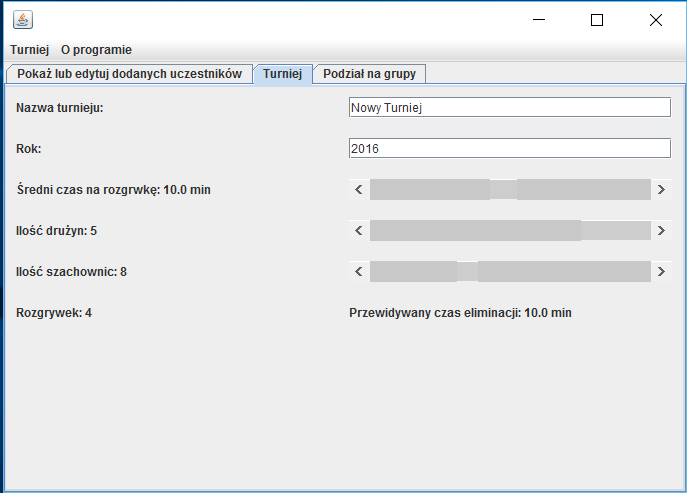
\includegraphics[width=10cm]{fig/7}
	\caption{Zakładka turniej}
	\label {fig:zakladka_turniej} 
\end{figure}
W zakładce "Podział na grupy" z menu "Sortowanie graczy" możemy wybrać sposób sortowania uczestników według kryteriów widocznych poniżej
\begin{figure}[H]
	\centering
	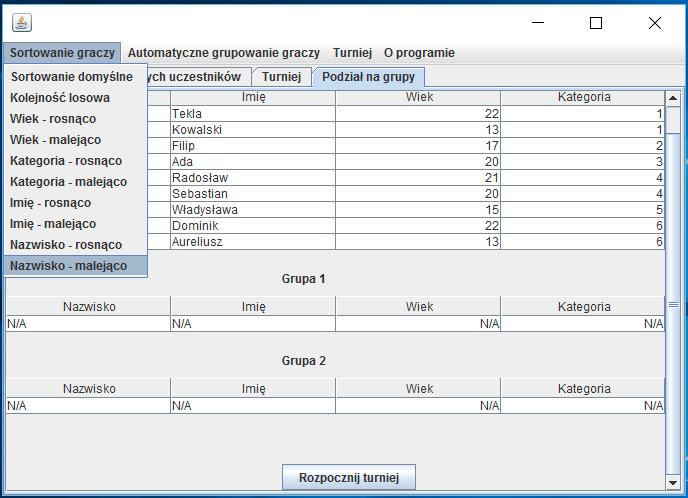
\includegraphics[width=10cm]{fig/8}
	\caption{Sposoby sortowania uczestników}
	\label {fig:Sposoby_sortowania_uczestnikow} 
\end{figure}
Zawodników możemy przydzielić do grup automatycznie
\begin{figure}[H]
	\centering
	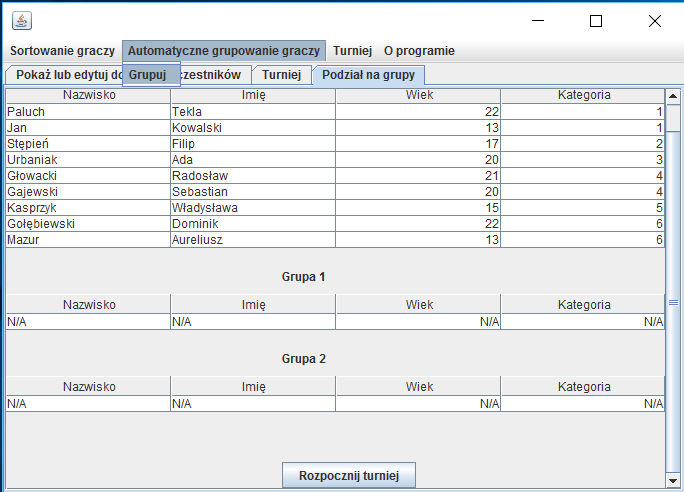
\includegraphics[width=10cm]{fig/9}
	\caption{Automatyczny przydział do grup}
	\label {fig:Automatyczny_przydzial_do_grup} 
\end{figure}
Zawodnika do grupy możemy przydzielić ręcznie klikając PPM i wybierając z listy grupę do której chcemy przydzielić uczestika
\begin{figure}[H]
	\centering
	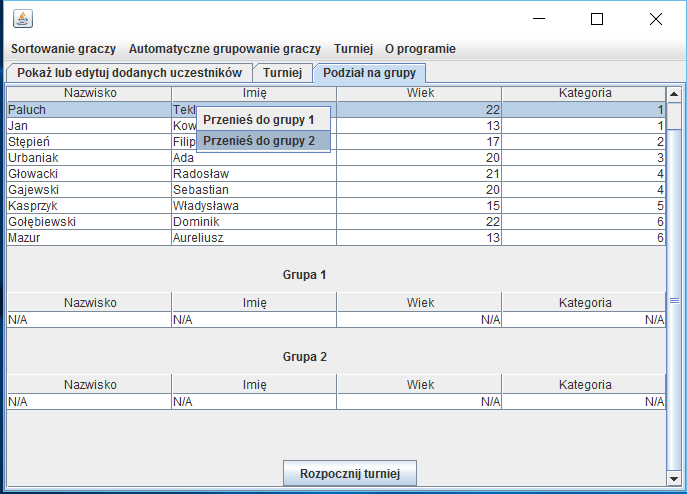
\includegraphics[width=10cm]{fig/10}
	\caption{Reczny przydział do grup}
	\label {fig:Reczny_przydzial_do_grup} 
\end{figure}
Jeżeli przydzielimy wszystkich zawodników do grup możemy rozpocząć turniej
\begin{figure}[H]
	\centering
	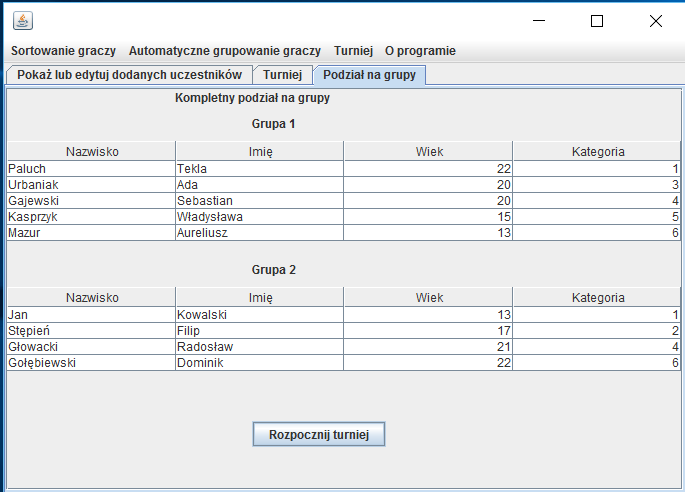
\includegraphics[width=10cm]{fig/11}
	\caption{Rozpoczęcie turnieju}
	\label {fig:rozpoczecie_turnieju} 
\end{figure}
Rozgrywki które mogą się odbyć zostają podświetlone na zielono\\
Zwycięzcę rozgrywki możemy wybrać z listy lub za pomocą skrótu klawiaturowego:
\begin{itemize}
	\item "b" - wygrywa kolor biały
	\item "c" - wygrywa kolor czarny
	\item "r" - remis
\end{itemize}

\begin{figure}[H]
	\centering
	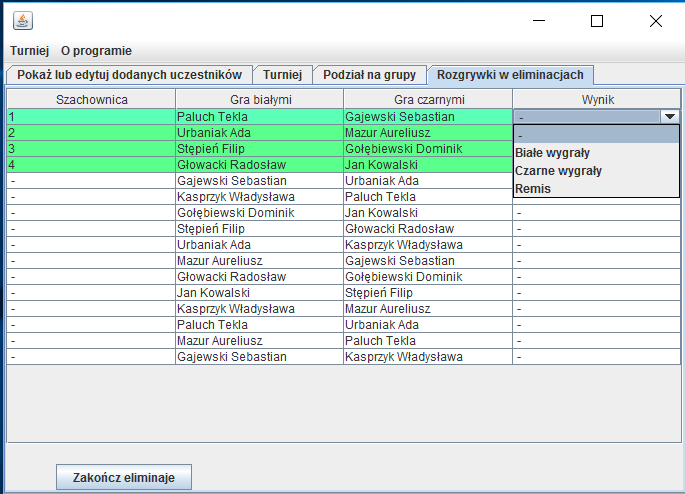
\includegraphics[width=10cm]{fig/12}
	\caption{Możliwe rozgrywki}
	\label {fig:mozliwe_rozgrywki} 
\end{figure}

\begin{figure}[H]
	\centering
	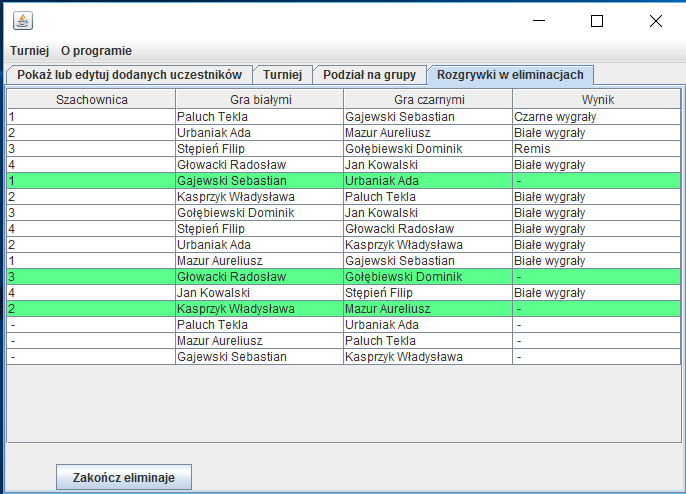
\includegraphics[width=10cm]{fig/13}
	\caption{Możliwe rozgrywki}
	\label {fig:mozliwe_rozgrywki_2} 
\end{figure}
Po ustaleniu wyników wszystkich rozgrywek możemy zakończyć eliminacje
\begin{figure}[H]
	\centering
	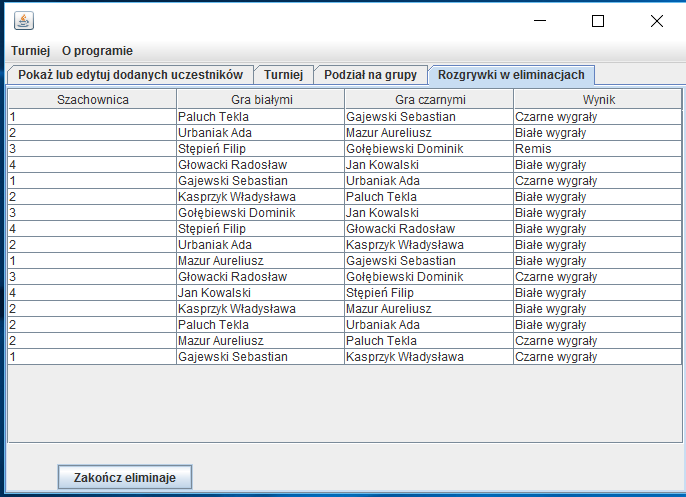
\includegraphics[width=10cm]{fig/14}
	\caption{Wybór zawodników do finału}
	\label {fig:wybor_zawodnikow_do_finalu} 
\end{figure}
Przechodzimy do zakładki "Wybór graczy do finałów"\\
Z każdej grupy musimy wybrać co najmniej jednego zawodnika który będzie brał udział w finale
\begin{figure}[H]
	\centering
	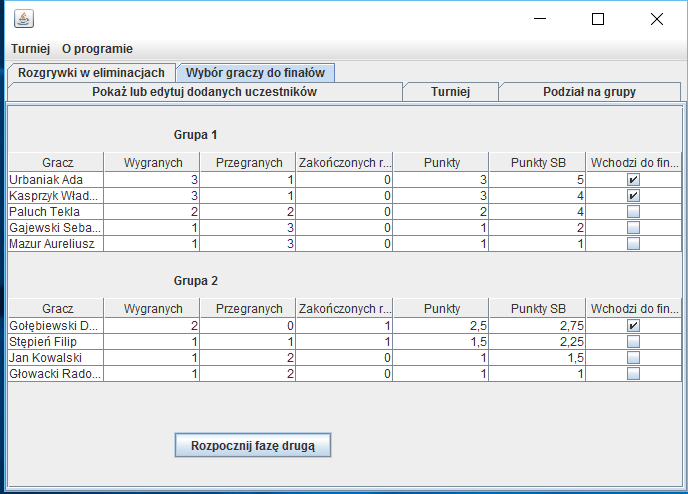
\includegraphics[width=10cm]{fig/15}
	\caption{Wybór graczy do finału}
	\label {fig:rozgrywka_finalowa_1} 
\end{figure}
Jeżeli zawodnicy którzy dostali się do finału grali ze sobą wcześniej, nie grają ponownie. Przyjęty zostaje wynik z poprzedniej rundy.
\begin{figure}[H]
	\centering
	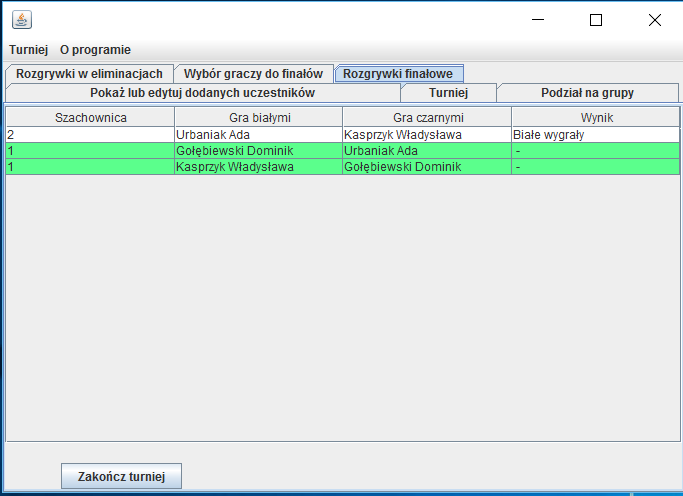
\includegraphics[width=10cm]{fig/16}
	\caption{Rozgrywki finałowe}
	\label {fig:rozgrywka_finalowa_2} 
\end{figure}

W zakładce "Wyniki turnieju" wyświetlone zostają wyniki z podziałem na miejsca
\begin{figure}[H]
	\centering
	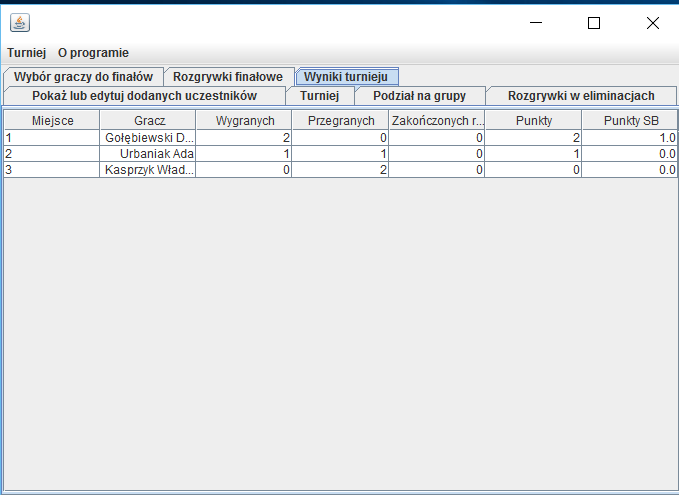
\includegraphics[width=10cm]{fig/17}
	\caption{Wyniki turnieju}
	\label {fig:wyniki_turnieju} 
\end{figure}
Po rozpoczęciu turnieju w zakładce "Pokaż lub edytuj dodanych uczestników" po kliknięciu PPM na wiersz z danymi uczestnika możemy wybrać opcję "Dyskwalifikuj". 
\begin{figure}[H]
	\centering
	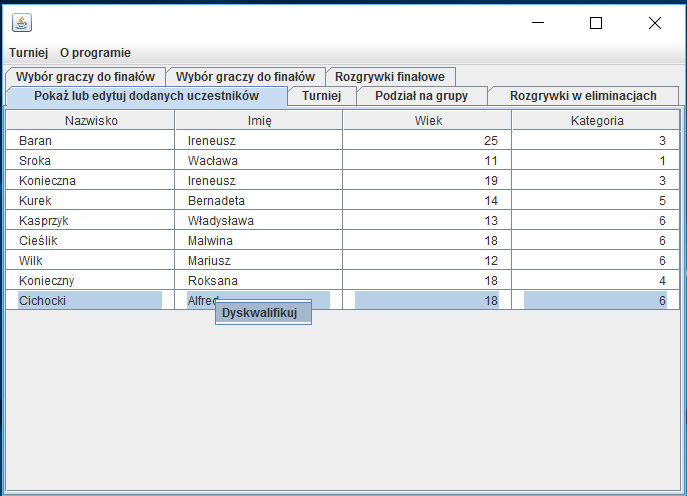
\includegraphics[width=10cm]{fig/18}
	\caption{Dyskwalifikacja zawodnika}
	\label {fig:dyskwalifikacja} 
\end{figure}
\textbf{Uwaga!!!} Z opcji dyskwalifikacji należy korzystać bardzo ostrożnie, tej operacji \textbf{nie} można cofnąć.
\begin{figure}[H]
	\centering
	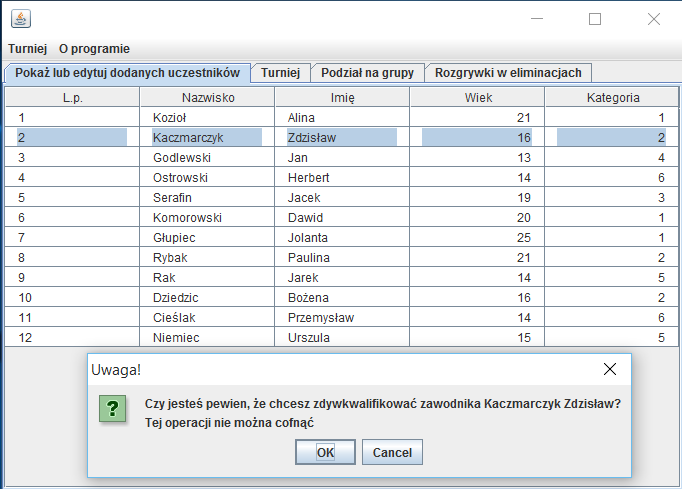
\includegraphics[width=10cm]{fig/19}
	\caption{Potwierdzenie dyskwalifikacji}
	\label {fig:dyskwalifikacja_potwierdzenie} 
\end{figure}
Jeżeli zawodnik rozegrał już jakieś pojedynki to nie zostają one anulowane a kolejne w których miał brać udział przegrywa walkowerem (przeciwnik dostaje 1 punkt), do nazwiska zawodnika zostaje dodane oznaczenie dyskwalifikacji "*d"
\begin{figure}[H]
	\centering
	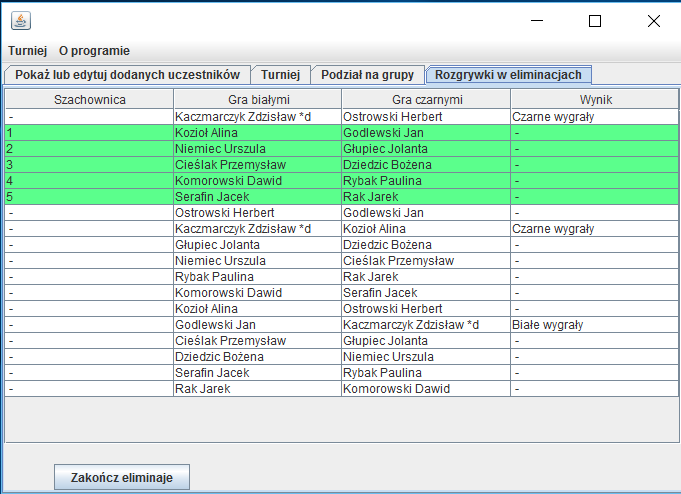
\includegraphics[width=10cm]{fig/20}
	\caption{Tabela wyników po dyskwalifikacji uczestnika}
	\label {fig:dyskwalifikacja_tabela} 
\end{figure}% obsługa programu
\chapter{Piotr Jabłoński,\\ Mirosława Pelc}



\textbf{Kod źródłowy z kompilatora Eclipse z komentarzami wygenerowany automatycznie.}
\url{file:./doc/index.html}%Piotr Jabłoński		
%\chapter{Mirosława Pelc}

Mirosława Pelc
Swing to biblioteka graficzna używana w języku programowania Java. To właśnie z tej biblioteki skorzystałam tworząc interfejs graficzny. Tworzenie GUI rozpoczęłam od „bazy” czyli okna głównego, zwanego JFrame w środowisku programistycznym. W tym celu należało rozszerzyć klasę odpowiadającą za okno główne dodając słowo extends a zaraz po nim JFrame.
\begin{verbatim}
public class MainWindow extends JFrame \{
private static final long serialVersionUID = -4321522332774571523L;

public static void main (String[]args)\{
new MainWindow().setVisible(true);
\}

public MainWindow() \{
setMinimumSize(new Dimension(700, 500));
setDefaultCloseOperation(JFrame.DISPOSE\_ON\_CLOSE);
setLayout(new BorderLayout());

setJMenuBar(Tools.aboutMenu(new JMenuBar(), MainWindow.this));

try \{
InputStream imgIS = getClass().getResourceAsStream("/szachy.png");
add(new JLabel(new ImageIcon(ImageIO.read(imgIS))), BorderLayout.CENTER);
\} catch (IOException e1) \{
e1.printStackTrace();
\}
\}
\}
\end{verbatim}
W powyższym kodzie ustawiłam rozmiar okna komendą setMinimumSize, dodałam obrazek startowy używając InputStream oraz ImageIcon. Stworzyłam pasek menu używając takich komponentów jak JMenu, JMenuItem, MenuBar. Tworzenie paska menu:
\begin{verbatim}
JMenu 	mnTurniej 	 = new JMenu("Turniej"),
mnOProgramie = new JMenu("O programie");
menuBar.add(mnTurniej);
menuBar.add(mnOProgramie);

JMenuItem 	mntmPomoc 		= new JMenuItem("Pomoc"),
dodajTurniej 	= new JMenuItem("Dodaj turniej"),
wybierzTurniej	= new JMenuItem("Wybierz turniej"),
mntmAutorzy 	= new JMenuItem("Autorzy"),
mntmOpis 		= new JMenuItem("Opis");

mntmPomoc.setAlignmentY(Component.TOP\_ALIGNMENT);

mnTurniej.add(dodajTurniej);
mnTurniej.add(wybierzTurniej);
mnOProgramie.add(mntmPomoc);
mnOProgramie.add(mntmAutorzy);
mnOProgramie.add(mntmOpis);

dodajTurniej.setAccelerator(KeyStroke.getKeyStroke(
java.awt.event.KeyEvent.VK\_F2, 0));
wybierzTurniej.setAccelerator(KeyStroke.getKeyStroke(
java.awt.event.KeyEvent.VK\_F3, 0));

dodajTurniej.addActionListener(e -> \{
frame.getContentPane().removeAll();
frame.add(new AddTPanel(frame), BorderLayout.CENTER);
frame.pack();
\});
wybierzTurniej.addActionListener(e -> \{
frame.getContentPane().removeAll();
frame.add(new ShowTPanel(frame), BorderLayout.CENTER);
frame.pack();
\});
// otwieranie pdf z instrukcją po wybraniu pomocy
mntmPomoc.addActionListener(e->\{
if(Desktop.isDesktopSupported()) \{
try \{
File myFile = new File("turniej.pdf");
Desktop.getDesktop().open(myFile);
\} catch (IOException ex) \{
System.out.println(e);
\}
\}
\});
\end{verbatim}
Dodane zostały skróty klawiszowe dla poszczególnych JMenuItem. Okno po wykonaniu czynności wygląda następująco:
\begin{figure}[H]
	\centering
	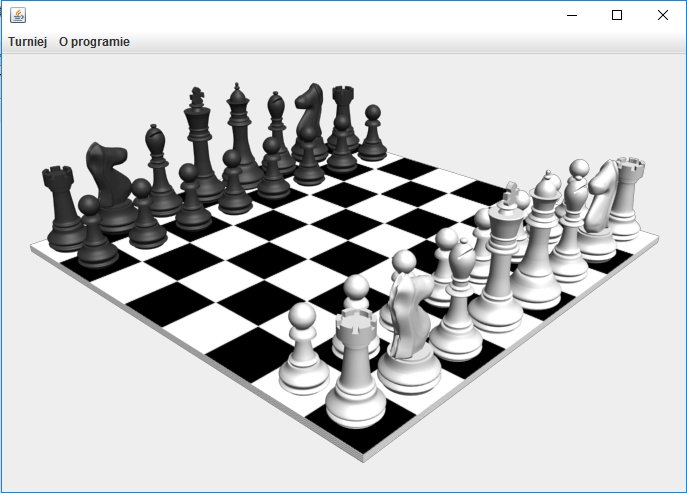
\includegraphics[width=10cm]{fig/m1}
	\caption{Skróty klawiszowe dla poszczególnych JMenuItem}
	\label {fig:JMenuItem} 
\end{figure}
Aby utworzyć nowy turniej potrzebnym było stworzenie nowego panelu, który łączy się z bazą danych. Oto jego kod:
\begin{verbatim}
package window;

import java.awt.Font;
import java.awt.event.ActionEvent;
import java.awt.event.ActionListener;
import java.util.Calendar;

import javax.swing.JButton;
import javax.swing.JFrame;
import javax.swing.JLabel;
import javax.swing.JPanel;
import javax.swing.JTextField;
import javax.swing.SwingConstants;

import model.Database;
import model.Tournament;
import panel.CompetitorTabbedPane;

/**
* Panel "nowy turniej"
*/
public class AddTPanel extends JPanel \{
private static final long serialVersionUID = -4930339429679727134L;
private JTextField textField;
private String nazwa;

public AddTPanel(final JFrame jframe)\{
setLayout(null);

JLabel nameTour = new JLabel("Nazwa turnieju");
nameTour.setFont(new Font("Consolas", Font.PLAIN, 16));
nameTour.setHorizontalTextPosition(SwingConstants.CENTER);
nameTour.setHorizontalAlignment(SwingConstants.CENTER);
nameTour.setBounds(100, 100, 484, 30);
add(nameTour);

textField = new JTextField();
textField.setBounds(100, 141, 484, 25);
textField.setColumns(10);
add(textField);

JButton addButton = new JButton("Utwórz");
addButton.setFont(new Font("Consolas", Font.PLAIN, 16));
addButton.setBounds(100, 293, 484, 30);
addButton.addActionListener(new ActionListener() \{
public void actionPerformed(ActionEvent e) \{
nazwa=textField.getText();
String year = String.valueOf(Calendar.getInstance().get(Calendar.YEAR));
Tournament t = new Tournament(null,nazwa,year,8,5,-1);
Database db = new Database();
db.insertOrUpdateTournament(t);
jframe.getContentPane().removeAll();
new CompetitorTabbedPane(t, jframe);
db.close();
\}
\});

// po naciśnięciu enter aktywuje się guzik DODAJ
jframe.getRootPane().setDefaultButton(addButton);

add(addButton);
\}
\}
\end{verbatim}
Panel zawiera takie komponenty jak JPanel, etykietę JLabel, pole tekstowe JTextField oraz guzik JButton. Stworzony panel wygląda następująco:
\begin{figure}[H]
	\centering
	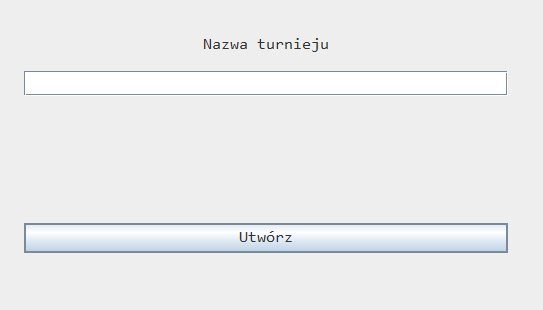
\includegraphics[width=10cm]{fig/m2}
	\caption{Komponenty panelu}
	\label {fig:panel} 
\end{figure}

Kolejnym krokiem było utworzenie panelu, który odpowiadałby za wybór wcześniej utworzonego turnieju. Kod tego panelu przedstawia się następująco:
\begin{verbatim}
package window;

import java.awt.Font;
import java.awt.event.ActionEvent;
import java.awt.event.ActionListener;

import javax.swing.JComboBox;
import javax.swing.JFrame;
import javax.swing.JLabel;
import javax.swing.JPanel;
import javax.swing.SwingConstants;

import model.Database;
import model.Tournament;
import panel.CompetitorTabbedPane;

/**
* Panel "dodaj turniej"
*/
public class ShowTPanel extends JPanel \{
private static final long serialVersionUID = -1094699102373510646L;
private Database db;

public ShowTPanel(final JFrame jframe) \{
db = new Database();
setLayout(null);

final JComboBox<String> comboBox = new JComboBox<String>();
comboBox.setFont(new Font("Consolas", Font.PLAIN, 15));
comboBox.setBounds(10, 100, 664, 30);

for(Tournament t: db.getTournaments())\{
String nazwa = t.getName();
comboBox.addItem(nazwa);
\}

comboBox.addActionListener (new ActionListener () \{
public void actionPerformed(ActionEvent e) \{
int sIndex = comboBox.getSelectedIndex();
jframe.getContentPane().removeAll();
new CompetitorTabbedPane(db.getTournaments().get(sIndex),jframe);
db.close();
\}
\});

add(comboBox);

JLabel wybierz = new JLabel("Wybierz turniej");
wybierz.setFont(new Font("Consolas", Font.PLAIN, 16));
wybierz.setHorizontalTextPosition(SwingConstants.CENTER);
wybierz.setHorizontalAlignment(SwingConstants.CENTER);
wybierz.setBounds(10, 59, 664, 30);
add(wybierz);		
\}	
\}
\end{verbatim}
Użyte komponenty to w tym przypadku etykieta JLabel oraz JComboBox czyli wysuwana lista, która zawiera nazwy zapisanych turniejów. Oto graficzna reprezentacja panelu wyboru turnieju:
\begin{figure}[H]
	\centering
	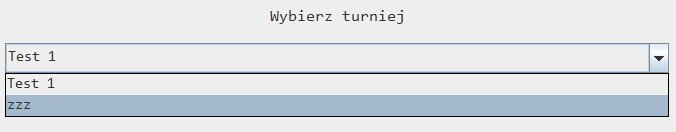
\includegraphics[width=10cm]{fig/m3}
	\caption{Graficzna reprezentacja panelu wyboru turnieju}
	\label {fig:G} 
\end{figure}

Po zatwierdzeniu utworzonego turnieju lub po wybraniu już istniejącego pojawia się okno odpowiadające za rozgrywki. Początkowo są trzy zakładki, których kod jest następujący:
\begin{verbatim}
public CompetitorTabbedPane(Tournament turniej, JFrame frame)\{
this.turniej = turniej;
this.DB = new Database();
showPanel = new ShowEditCompetitorPanel(turniej, DB);
tournamentPanel = new TournamentPanel(turniej, DB);
[…]
groupsPanel = new GroupsPanel(turniej, DB, tStartlistener);
setMenu(frame);
tabbedPane.add(Strings.showOrEditComp, showPanel);
tabbedPane.add(Strings.tournament, tournamentPanel);
tabbedPane.add(Strings.prepGroups, groupsPanel);
tabbedPane.addChangeListener((e) -> \{
int i = tabbedPane.getSelectedIndex();
if(i==0) showPanel.setData();
if(i==1) tournamentPanel.setSBBounds();
if(i==2) groupsPanel.initComponents();
if(i==3) gamesPanel.initComponents();
if(i==5) finaleGamesPanel.initComponents();
comp.setVisible( turniej.isPlayersEditAllowed() \&\& i==0);
group.setVisible(turniej.isPlayersEditAllowed() \&\& i==2 );
sort.setVisible(i==2);
\});

frame.add(tabbedPane);
setVisible(true);
\end{verbatim}
Użyty został komponent JTabbedPane, który odpowiada za panel z zakładkami. 

Jak można łatwo zauważyć, program ma wiele tabelek. JTable to kolejny komponent biblioteki Swing. Przykładowe tabele:
\begin{verbatim}
private JTable table;
[…]
table = new EditCompetitorJTable();
[…]
public class EditCompetitorJTable extends JTable \{
private static final long serialVersionUID = -9074329149984999956L;

public EditCompetitorJTable() \{
super();
setIntercellSpacing(new Dimension(25, 2));
setRowHeight(20);
setModel(new EditCompetitorTableModel());

setSelectionMode(javax.swing.ListSelectionModel.SINGLE\_SELECTION); 
// pole tekstowe akceptujące tylko znaki a-Z, - i spację
final JTextField jtf = new JTextField(new MyPlainDocument(), null, 0);
// przy rozpoczęciu edyji zaznaczenie wszystkiego
jtf.addFocusListener(new FocusAdapter() \{
@Override
public void focusGained(FocusEvent e) \{
jtf.selectAll();
\}
\});

// dla pól imię i nazwisko ustawiony edytor na podstawie powyższego pola tekstowego 
columnModel.getColumn(1).setCellEditor(new DefaultCellEditor(jtf));
columnModel.getColumn(2).setCellEditor(new DefaultCellEditor(jtf));
columnModel.getColumn(4).setCellEditor(new DefaultCellEditor(
new JComboBox<Integer>(new Integer[]\{1,2,3,4,5,6\})
));
\}

// po przejśiu do komórki (również tabulatorem) rozpoczęcie edycji
public void changeSelection(int row, int column, boolean toggle, boolean extend) \{
super.changeSelection(row, column, toggle, extend);
if(editCellAt(row, column)) \{
getEditorComponent().requestFocusInWindow();
\}
\}
\}
\end{verbatim}
\begin{verbatim}
JTable table = new JTable(new MyTableModel());
table.getColumnModel().getColumn(3).setCellEditor(new DefaultCellEditor(
new JComboBox<String>(new String[] \{Strings.notPlayedYet, Strings.whiteWon, Strings.blackWon, Strings.tie\})
));
table.setDefaultRenderer(String.class, new MyCellRenderer());
add(new JScrollPane(table));
\end{verbatim}
A oto kod odpowiadający za formatowanie JTable
\begin{verbatim}
public class EditCompetitorJTable extends JTable \{
private static final long serialVersionUID = -9074329149984999956L;

public EditCompetitorJTable() \{
super();
setIntercellSpacing(new Dimension(25, 2));
setRowHeight(20);
setModel(new EditCompetitorTableModel());

setSelectionMode(javax.swing.ListSelectionModel.SINGLE\_SELECTION); 
// pole tekstowe akceptujące tylko znaki a-Z, - i spację
final JTextField jtf = new JTextField(new MyPlainDocument(), null, 0);
// przy rozpoczęciu edyji zaznaczenie wszystkiego
jtf.addFocusListener(new FocusAdapter() \{
@Override
public void focusGained(FocusEvent e) \{
jtf.selectAll();
\}
\});

// dla pól imię i nazwisko ustawiony edytor na podstawie powyższego pola tekstowego 
columnModel.getColumn(1).setCellEditor(new DefaultCellEditor(jtf));
columnModel.getColumn(2).setCellEditor(new DefaultCellEditor(jtf));
columnModel.getColumn(4).setCellEditor(new DefaultCellEditor(
new JComboBox<Integer>(new Integer[]\{1,2,3,4,5,6\})
));
\}

// po przejśiu do komórki (również tabulatorem) rozpoczęcie edycji
public void changeSelection(int row, int column, boolean toggle, boolean extend) \{
super.changeSelection(row, column, toggle, extend);
if(editCellAt(row, column)) \{
getEditorComponent().requestFocusInWindow();
\}
\}
\}
\end{verbatim}

Aby nie powielać kodu przy formatowaniu modelu JTable stworzyłam klasę abstrakcyjną modelu rozszerzającą AbstractTableModel, którą przypisuję do tabeli.
\begin{verbatim}
protected abstract class MyTableModel extends AbstractTableModel \{
private static final long serialVersionUID = -8079013606990307646L;
final String[] columnNames = \{Strings.board, Strings.playsWithWhite, Strings.playsWithBlack, Strings.score\};
@Override
public Class<?> getColumnClass(int columnIndex) \{
return String.class;
\}
@Override
public int getColumnCount() \{
return 4;
\}
@Override
public String getColumnName(int columnIndex) \{
return columnNames[columnIndex];
\}
@Override
public int getRowCount() \{
return singleGames.size();
\}
@Override
public Object getValueAt(int row, int col) \{
SingleGame sg = singleGames.get(row);
if(col==0 \&\& sg.getBoard()==-1) return " - ";
if(col==0) return sg.getBoard()+1;
if(col==1) return competitorMap.get(sg.getCompetitorW());
if(col==2) return competitorMap.get(sg.getCompetitorB());
if(col==3) \{
if(sg.getScore()==0) return Strings.notPlayedYet;
if(sg.getScore()==1) return Strings.whiteWon;
if(sg.getScore()==2) return Strings.blackWon;
if(sg.getScore()==3) return Strings.tie;
\}
return null;
\}
public abstract void setValueAt(Object aValue, int row, int col);
\}
\}
\end{verbatim}

W celu ułatwienia użytkownikowi programu przydzielanie zawodników do szachownic, komórki  JTable zostały pokolorowane. Oto jak wygląda to w kodzie programu:
\begin{verbatim}
final void recalcColors() \{
currentlyPlayedGames = new ArrayList<>(turniej.getBoards());
currentlyPlayedGames.clear();;
List<Integer> 	playingCompetitors 	= new ArrayList<>(2*turniej.getBoards()),
freeBoards 			= new LinkedList<>();
for(int i=0; i<turniej.getBoards(); ++i) freeBoards.add(i);
for(SingleGame sg : singleGames.stream().filter(g->g.getScore()==0\&\&g.getBoard()>=0)
.collect(Collectors.toList()))\{
freeBoards.remove(sg.getBoard());
playingCompetitors.add(sg.getCompetitorW());
playingCompetitors.add(sg.getCompetitorB());
currentlyPlayedGames.add(sg);
\};
for(SingleGame sg : singleGames.stream().filter(g->g.getScore()==0\&\&g.getBoard()<0)
.collect(Collectors.toList()))\{
if(freeBoards.isEmpty()) break;
if(!playingCompetitors.contains(sg.getCompetitorW()) \&\&
!playingCompetitors.contains(sg.getCompetitorB())) 
\{
int board = freeBoards.get(0);
sg.setBoard(board);
freeBoards.remove(0);
playingCompetitors.add(sg.getCompetitorW());
playingCompetitors.add(sg.getCompetitorB());
currentlyPlayedGames.add(sg);
\}	
\};
sortGames();
\}
\end{verbatim}
\begin{verbatim}
package res;

import java.awt.Color;

public final class Colors \{
public final static Color 
selInProgress 	= Color.decode("\#5BFFB5"),
selNormal		= Color.decode("\#84D4FF"),
InProgress		= Color.decode("\#5BFF8C"),
normal 			= Color.decode("\#FFFFFF");
\}
\end{verbatim}

Druga zakładka w oknie turnieju to edycja turnieju, czyli: zmiana tytułu, ustawienie roku rozgrywania turnieju, suwaki odpowiedzialne za ilość szachownic, czas rozgrywki, ilość grup. Użyte komponenty to etykieta JLabel, pole tekstowe JTextField, suwak ScrollBar. Layout panelu ustawiony jest na GridLayout(0,2,…) co oznacza, że panel podzielony jest na dwie kolumny a komponenty dodawane są raz do jednej kolumny, raz do drugiej. Oto kod TournamentPanel:
\begin{verbatim}
package panel;

import java.awt.BorderLayout;
import java.awt.Component;
import java.awt.GridLayout;
import java.awt.Scrollbar;

import javax.swing.JLabel;
import javax.swing.JPanel;
import javax.swing.JTextField;
import javax.swing.border.EmptyBorder;
import javax.swing.event.DocumentEvent;
import javax.swing.event.DocumentListener;

import model.Database;
import model.Tournament;
import res.Strings;
import tools.MyPlainDocument;
import tools.Simulator;

/**
* Zakładka danych o turnieju
*/
public class TournamentPanel extends JPanel\{
private static final long serialVersionUID = -3657045958131642437L;
private final Tournament turniej;
private final Database DB;
private final JLabel nameL, yearL, sgTimeL, groupsL, boardsL, stats1L, stats2L;
final JTextField nameTF, yearTF;
final Scrollbar groupsSB, sgTimeSB, boardsSB;
final JPanel panel = new JPanel();
/**
* @param t - id turnieju
* @param db - baza danych
*/
public TournamentPanel(Tournament t, Database db)\{
this.turniej = t;
this.DB = db;
nameL 	= new JLabel("Nazwa turnieju: ");
yearL 	= new JLabel("Rok: ");
sgTimeL = new JLabel(Strings.sgTimeT+"10 min");
groupsL = new JLabel(Strings.groupsT+"2");
boardsL = new JLabel(Strings.boardsT);
stats1L = new JLabel(Strings.gamesT);
stats2L = new JLabel(Strings.timeRRET);
nameTF 	= new JTextField();
yearTF  = new JTextField();
groupsSB 	= new Scrollbar(Scrollbar.HORIZONTAL, 2, 1, 2, 9+1);
sgTimeSB 	= new Scrollbar(Scrollbar.HORIZONTAL, 20, 4, 2, 40+4);
boardsSB 	= new Scrollbar(Scrollbar.HORIZONTAL, 8, 1, 2, 20+1);

setLayout(new BorderLayout());
setBorder(new EmptyBorder(10, 10, 10, 10));
panel.setLayout(new GridLayout(0, 2, 10, 20));
add(panel, BorderLayout.NORTH);
nameTF.setDocument(new MyPlainDocument());
yearTF.setDocument(new MyPlainDocument());

setComponentsActions();

Component[] cs = \{
nameL, nameTF, yearL, yearTF, sgTimeL, sgTimeSB, groupsL, groupsSB, boardsL, boardsSB, stats1L, stats2L
\};
for(Component c : cs) panel.add(c);

nameTF.setText(turniej.getName());
yearTF.setText(turniej.getYear());
setSBBounds();
recalcStats();
\}

private void setComponentsActions() \{
nameTF.getDocument().addDocumentListener(new MyDocumentListener() \{			
@Override
public void action() \{
turniej.setName(nameTF.getText());
DB.insertOrUpdateTournament(turniej);
\}
\});
yearTF.getDocument().addDocumentListener(new MyDocumentListener() \{
@Override
public void action() \{
turniej.setYear(yearTF.getText());
DB.insertOrUpdateTournament(turniej);
\}
\});
groupsSB.addAdjustmentListener(e -> \{
if(!turniej.isPlayersEditAllowed()) \{
groupsSB.setValue(turniej.getRounds());
return;
\}
int g = groupsSB.getValue();
turniej.setRounds(g);
DB.insertOrUpdateTournament(turniej);
recalcStats();
\});
boardsSB.addAdjustmentListener(e -> \{
if(!turniej.isPlayersEditAllowed()) \{
boardsSB.setValue(turniej.getBoards());
return;
\}
int g = boardsSB.getValue();
turniej.setBoards(g);
DB.insertOrUpdateTournament(turniej);
recalcStats();
\});
sgTimeSB.addAdjustmentListener(e -> \{
recalcStats();
\});
\}

private abstract class MyDocumentListener implements DocumentListener \{
public abstract void action();
@Override public final void removeUpdate(DocumentEvent e) \{ action(); \}
@Override public final void insertUpdate(DocumentEvent e) \{ action(); \}
@Override public final void changedUpdate(DocumentEvent e)\{ action(); \}
\}

public void recalcStats() \{ // TODO - poprawić przewidywany czas turnieju
groupsL.setText(Strings.groupsT+groupsSB.getValue());
boardsL.setText(Strings.boardsT+boardsSB.getValue());
sgTimeL.setText(Strings.sgTimeT+(sgTimeSB.getValue()/2f)+" min");
int graczy = DB.getCompetitors(turniej.getId()).size();
if(turniej.getBoards()<1 || graczy<2) return;
float czasSG = sgTimeSB.getValue()/2f;
int grup = groupsSB.getValue();
int rozgrywek = Simulator.rozgrywek\_eliminacje(graczy, grup);
stats1L.setText(Strings.gamesT+String.valueOf(rozgrywek));
int gier\_naraz = (int)Math.min(Math.floor(graczy/2), turniej.getBoards());
stats2L.setText(Strings.timeRRET+Math.ceil(rozgrywek/gier\_naraz)*czasSG+" min");
\}
public void setSBBounds() \{
int graczy = DB.getCompetitors(turniej.getId()).size();
groupsSB.setMinimum(2);
groupsSB.setMaximum((int)Math.ceil(graczy/2)+2);
groupsSB.setValue(turniej.getRounds());
recalcStats();
\}
\}
\end{verbatim}
Poniższy rysunek przedstawia kod po skompilowaniu: 
\begin{figure}[H]
	\centering
	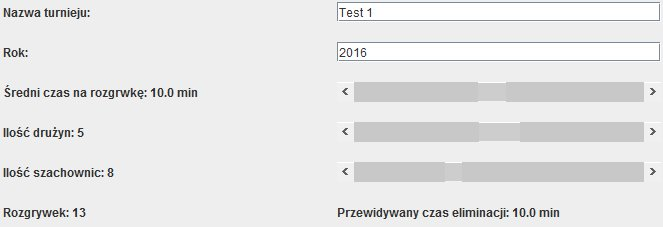
\includegraphics[width=10cm]{fig/m4}
	\caption{Edycja turnieju}
	\label {fig:EdycjaTurnieju} 
\end{figure}

Program nie dopuszcza do zaistnienia pewnych zdarzeń, jeśli użytkownik wprowadzi błędne dane lub dobierze zawodników źle w grupy wówczas wyskoczy błąd. Za wiadomości o błędach odpowiada JOptionPane. Na potrzemy programu stworzyłam kilka wiadomości o błędach. Kod:
\begin{verbatim}
package tools;

import javax.swing.JOptionPane;

import model.Competitor;

/**
* Definiuje okna błędów, ostrzeżeń oraz informacji
*/
public class Dialogs \{
public static void bladBazy() \{
JOptionPane.showMessageDialog(
null, 
"Błąd odczytu / zapisu", 
"Błąd bazy", 
JOptionPane.ERROR\_MESSAGE);
\}

public static void graczBezGrupy() \{
JOptionPane.showMessageDialog(
null, 
"Aby móc rozpocząć turniej, każdy gracz musi być przydzielony do grupy", 
"Gracz bez grupy", 
JOptionPane.ERROR\_MESSAGE);
\}

public static void nierownomiernyPodzial(int min, int max) \{
JOptionPane.showMessageDialog(
null, 
"Największa grupa: "+max+" uczestników, \textbackslash\{\}n"+
"Najmniejsza grupa: "+min+" uczestników \textbackslash\{\}n"+
"Różnica pomiędzy tymi wartościami nie może być większa od 1", 
"Nierównomierny podział", 
JOptionPane.ERROR\_MESSAGE);
\}

public static void gryBezWyniku() \{
JOptionPane.showMessageDialog(
null, 
"Aby zakończyć eliminacje, wszystkie gry tej fazy muszą być ukończone", 
"Nieukończone rozgrywki", 
JOptionPane.ERROR\_MESSAGE);
\}

public static void autorzy() \{
JOptionPane.showMessageDialog(
null,
"Autorzy: \textbackslash\{\}n"+
"Piotr Jabłoński\textbackslash\{\}n"+
"Mirosława Pelc\textbackslash\{\}n"+
"Mariusz Lorek",
"Autorzy", JOptionPane.UNDEFINED\_CONDITION);
\}

public static void opis() \{
JOptionPane.showMessageDialog(
null,
"Program powstał w ramach zaliczenia Zespołowych Przedsięwzięć Inżynierskich"+
"na Państwowej Wyższej Szkole Zawodowej w Nowym Sączu.\textbackslash\{\}nProwadzący przedmiot: "+
"dr Antoni Ligęza\textbackslash\{\}nProgram obsługuje turniej szachowy odbywający się podczas "+
"Małopolskiej Nocy Naukowców.",
"Opis", JOptionPane.UNDEFINED\_CONDITION);
\}

/**
* @return Czy kontynuować mimo ostrzeżenia
*/
public static boolean niktZGrupyDoFinalow() \{
int r = JOptionPane.showConfirmDialog(
null, 
"Istnieje grupa, w której nie wybrano graczy przechodzących do finału. Kontynuować?",
"Uwaga!",
JOptionPane.OK\_CANCEL\_OPTION);
return r==JOptionPane.OK\_OPTION;
\}

/**
* @return Czy na pewno zdyskwalifikowac
*/
public static boolean czyZdyskwalifikowac(Competitor c) \{
int r = JOptionPane.showConfirmDialog(
null, 
"Czy jesteś pewien, że chcesz zdywkwalifikować zawodnika "+c+"?\textbackslash\{\}nTej operacji nie można cofnąć",
"Uwaga!",
JOptionPane.OK\_CANCEL\_OPTION);
return r==JOptionPane.OK\_OPTION;
\}
\}
\end{verbatim}
Tak wygląda przykładowe okno informujące o błędzie:
\begin{figure}[H]
	\centering
	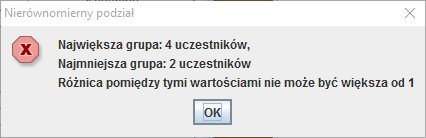
\includegraphics[width=10cm]{fig/m5}
	\caption{Okno informujące o błędzie}
	\label {fig:OknoBledu} 
\end{figure}

Podczas generowania losowych graczy imiona i nazwiska pobierane są z plików imiona.txt oraz nazwiska.txt, które zawarte są w pliku jar. Poniżej pokazałam jak to się odbywa w programie:
\begin{verbatim}
public static Competitor RandomPlayer() throws IOException \{
Random rn = new Random();
int a = 10+rn.nextInt(10)+rn.nextInt(10);
int c = rn.nextInt(6)+1;

int randomInt = rn.nextInt(300);
String imie = null, nazwisko = null;

InputStream imionaIS = JFrame.class.getResourceAsStream("/imiona.txt");
InputStream nazwiskaIS = JFrame.class.getResourceAsStream("/nazwiska.txt");

imieReader = new BufferedReader(new InputStreamReader(imionaIS, "UTF-8"));
nazwiskoReader = new BufferedReader(new InputStreamReader(nazwiskaIS, "UTF-8"));

imieReader.mark(0);
nazwiskoReader.mark(0);

do \{
imieReader.reset();
nazwiskoReader.reset();
for (int i = 0; i < randomInt; i++) \{
imie = imieReader.readLine();
nazwisko = nazwiskoReader.readLine();
\}
\} while(imie==null || nazwisko==null || (imie.endsWith("a") \&\& nazwisko.endsWith("ki")));
return new Competitor(null, imie, nazwisko, a, c, false, null);
\}
\end{verbatim}

%Mirosława Pelc
%\chapter{Mariusz Lorek}
%Mariusz Lorek
%%Usuwa numeracje z naglowka. Zapewnia  dodanie do spisu tresci
\setcounter{secnumdepth}{-1}


%Gdy mamy dużą bibliografię to możemy wybierać pozycje,
%które cytujemy
%\nocite{ad-tg-80}

%Dodaje wszystkie pozycje z bibliografii
%\nocite{*}

%Po kazdym dodaniu nowej pozycji bibliograficznej
%z katalogu glownego uruchom: bibtex pracadyp
%\bibliographystyle{pdplain}
%\bibliography{tex/pracadyp}

\begin {thebibliography}{11}
\bibitem{Balcerzak2005} Balcerzak J., Pansiuk J.: \emph{Wprowadzenie do kartografii matematycznej}, Warszawa, OWPW~2005.
\bibitem{Barrett} Barrett R. i inni: \emph{Templates for the Solution of Linear Systems: Building Blocks for Iterative Methods1}, wersja elektorniczna Mathematics http://www.siam.org/books.
\bibitem{bjork} Bjork A., Dahlquist G.: \emph{Numerical Methods in Scientific Computing}, Philadelphia, SIAM~2002.
\bibitem{CCITTG4}CCITT, \emph{Facsimile Coding Schemes and Coding Control Functions for Group 4 Facsimile
Apparatus, Recommendation T.6, Volume VII, Fascicle VII.3, Terminal Equipment and
Protocols for Telematic Services, The International Telegraph and Telephone Consultative Committee (CCITT)}, Geneva, CCITT~1985.
\bibitem{drwal:mathematica2000} Drwal G, i in., \emph{Mathematica 4}, Gliwice, WPKJS~200.
\bibitem{Gdowski1982} Gdowski B.: \emph{Elementy geometrii rózniczkowej w zadaniach}, Warszawa, PWN~1982.
\bibitem{Gotlib2007} Gotlib D., Iwaniak A., Olszewski R.: \emph{GIS obszary zastosowań}, Warszawa, PWN~2007.
\bibitem{INTERGRAPHFileFormat1994} INTERGRAPH: \emph{INTERGRAPH RASTER FILE FORMAT REFERENCE GUIDE}, Alabama, Intergraph Corporation~1994.
\bibitem{Januszewski2006} Januszewski J.: \emph{Systemy satelitarne GPS, Galileo i inne}, Warszawa, PWN~2006.
\bibitem{kielbasinski1992}: Kiełbasiński A., Schwetlick H.: \emph{Numeryczna algebra liniowa}, Warszawa, WNT~1992.
\bibitem{Kincaid2006} Kincaid D.: \emph{Analiza numeryczna}, Warszawa, WNT~2006.
\bibitem{Lamparski2001}Lamparski J.: \emph{Navstar GPS od teorii do praktyki}, Olsztyn, WUW-M~2001.
\bibitem{Levine1994} Levine J.: \emph{Programowanie plików graficznych w C/C++}, New York, Wiley~1994.
\bibitem{Longley2006} Longley P. i inni: \emph{GIS teoria i praktyka}, Warszawa, PWN~2006.
\bibitem{GML:opengis} Open Geospatial Consortium Inc.: \emph{OpenGIS Geography Markup Language (GML) Encoding Standard, Version: 3.2.1},  OGC~2007.
\bibitem{GML:opengisimplemntation} Open Geospatial Consortium Inc.: \emph{OpenGIS® Geography Markup Language (GML) Implementation Specification}, OGC~2004.
\bibitem{Opera2002} Opera J.: \emph{Geometria róniczkowa i jej zastosowania}, Warszawa, PWN~2002.
\bibitem{Poczobut1982Geogeza} Odlanicki-Poczobut M.: \emph{Geodezja}, PPWK~1982.
\bibitem{Li2007}Li Y. i inni: \emph{GML Topology Data Storage Schema Design}, Chiba University~2007.
\bibitem{li2004GMLstorage}Li Y., Li J., Zhou S.: \emph{GML Storage}, A Spatial Database Approach,ER (Workshops), str 55-66, 2004.
\bibitem{Sayood2002} Sayood K.: \emph{Kompresja danych}, Warszawa, Rm~2002.
\bibitem{G52003} \emph{The Technical Instruction G-5, The Ground Cadastre and Buildings, The Main Surveying and
Cartographic Bureau}, Warszawa 2003.



\end {thebibliography}


\listoffigures

%\listoftables
\end{document}